% Chapter Template

\chapter{Simulation} % Main chapter title

\noindent\textbf{\large Contents:}

\noindent\hrulefill
\noindent\startcontents[chapters]
\noindent\printcontents[chapters]{}{1}{}
\noindent\hrulefill

\label{Chapter2}% Change X to a consecutive number; for referencing this chapter elsewhere, use \ref{ChapterX}

The simulation portion of this research was to find what the response in the focal plane of our science image would
be if one or more of the segments was out of phase from the rest.  In order to do this, one segment will be isolated
at a time and each of the three aberrations will be applied to it (Piston, Tip, or Tilt).  All 21 combinations for
P/T/T for all seven segments will be put into a matrix called the response matrix (RM).  All coding was done in
python using the python package HCIpy made in house at Leiden University \cite{por2018hcipy}.  This section will go
into the process of building the response matrix as well as preparing the FPWFS.


\section{Response Matrix}
\label{sec:RM}

At the beginning of this project I was given two files, both of which were representative of the GMT pupil.  One was
a binary amplitude mask of the GMT pupil (Figure \ref{fig:amp_mask} and the other was the phase mask (Figure
\ref{fig:phase_mask}) that would be induced by the vAPP.  Both masks have the asymmetry discussed in \S
\ref{sec:vAPP} in order to detect all of the modal basis set in the focal plane.

\begin{figure}[H]
\centering
\begin{subfigure}{.5\textwidth}
  \centering
  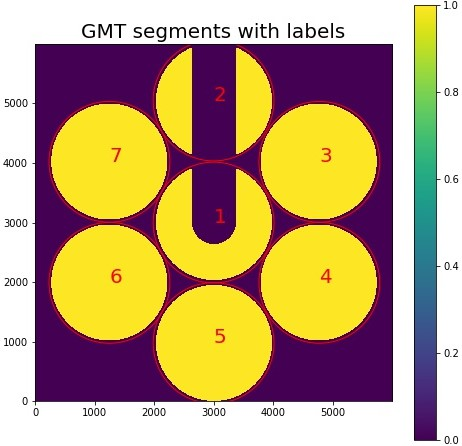
\includegraphics[width=6cm]{Figures/GMT_seg_choice.jpg}
  \caption{Amplitude mask of the GMT pupil.  Each segment is labeled 1-7 for which segment is to be isolated by the code.}
  \label{fig:amp_mask}
\end{subfigure}%
\begin{subfigure}{.5\textwidth}
  \centering
  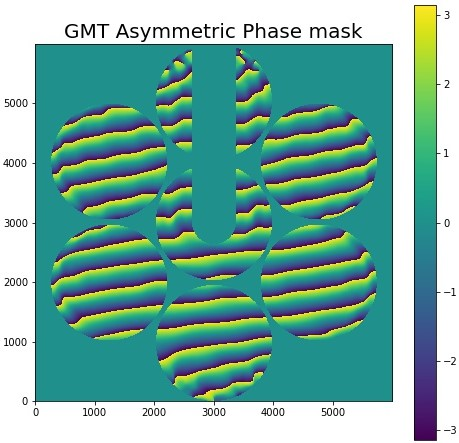
\includegraphics[width=6cm]{Figures/gmt_phase_mask.jpg}
  \caption{GMT phase mask that will be induced by the vAPP.  Each segment has a sinusoidal wave going across each segment.}
  \label{fig:phase_mask}
\end{subfigure}
\caption{Asymmetric pupil planes used for simulation of the GMT FPWFS test}
\label{fig:asym_pupils}
\end{figure}


In order to apply aberrations to a segment, I needed to isolate one of the segments.  The code makes a circle of
ones roughly the shape of the segment, and zeros across the rest of the array. When the circle mask was multiplied
by Figure \ref{fig:amp_mask} we get the segment isolated (Figure \ref{fig:single_seg}).  With the segment isolated,
we now want to add an aberration to this segment.  As an example I will look at tilt.  With the segment isolated,
the code generates a tip across the entire image and then makes sure that the values range from -1 to 1 only for the
segment (Figure \ref{fig:tilt_seg}).  

\begin{figure}[H]
\centering
\begin{subfigure}{.5\textwidth}
  \centering
  
\includegraphics[width=6.5cm]{Figures/isolated_seg.png}
  \caption{Segment 4 isolated by the code.}
  \label{fig:single_seg}
\end{subfigure}%
\begin{subfigure}{.5\textwidth}
  \centering
  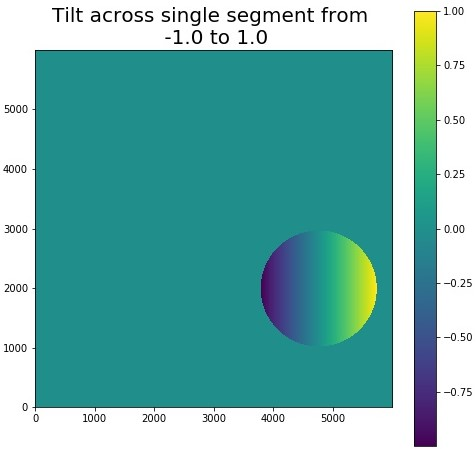
\includegraphics[width=6.5cm]{Figures/tip_single_seg.jpg}
  \caption{Isolated segment with a tilt applied to it.}
  \label{fig:tilt_seg}
\end{subfigure}
\caption{Isolated segment manipulation}
\label{fig:isolated_seg}
\end{figure}

However, we want to know the physical values of the tilt rather than just applying a tilt to the segment.  In order
to do this, we will apply an optical path difference (OPD) between the unaberrated segment and the segment with
aberration.  The phase difference is given by:

\begin{equation}
    \phi = 2 \pi \times \frac{d}{\lambda}
    \label{eq:OPD}
\end{equation}

Where $d$ is a distance in nanometers and $\lambda$ is the operation wavelength.  In this case, $\lambda = 532$nm. 
This is because the vAPP used on our optical testbed was tuned for lasers operating at 532nm.  For simplicity, the
code constructed the matrix for an OPD of 1nm so Equation \ref{eq:OPD} is simplified to $\phi = 2 \pi / \lambda$. 
With the phase difference calculated, it is multiplied by the tilt array (Figure \ref{fig:tilt_seg}), to give us a
segment with the appropriate values.  With the modification done to the segment, next step is to recombine the
aberration (Figure \ref{fig:tilt_seg}), amplitude mask (Figure \ref{fig:amp_mask}, as well as the phase mask (Figure
\ref{fig:phase_mask}).  To do this, I used the following equation:

\begin{equation}
    I = A \times e^{i \phi}
    \label{eq:intensity}
\end{equation}

Where $I$ is intensity, $A$ is the amplitude (Figure \ref{fig:amp_mask}) and $\phi$ is the phase of light (Figure
\ref{fig:phase_mask}).  However, just using Equation \ref{eq:intensity} will give a unaberrated image.  Using the
OPD, we combine the aberration and unaberrated pupil plane in the exponential because these are phase differences. 
This is done for each of the three PSFs that come from the vAPP.  So we now have three different intensity
equations:

\begin{align}
    & I_{top} = A \times e^{(i \cdot (\phi_{ab} + \phi))} \label{eq:top_PSF} \\
    & I_{leakage} = A \times 0.1 \times e^{i \phi_{ab}} \label{eq:leak_PSF} \\
    & I_{bottom} = A \times e^{(-i \phi) + (i \phi_{ab})} \label{eq:bottom_PSF}
\end{align}

Here $\phi_{ab}$ is the phase aberration we previously made, and the multiplication factor of 0.1 for Equation
\ref{eq:leak_PSF} is an intensity approximation of the leakage term.  With all of these combined we get a pupil
plane as shown in Figure \ref{fig:tilt_pupil}.  However, we want to propagate each PSF separately and then add up
the intensities.  Propagation is done with an inbuilt function of HCIpy called FraunhoferPropagator
\cite{por2018hcipy}.  After each PSF is propagated and added together in the focal plane, we get an image like that
in Figure \ref{fig:tilt_focal}.

\begin{figure}[H]
\centering
\begin{subfigure}{.5\textwidth}
  \centering
  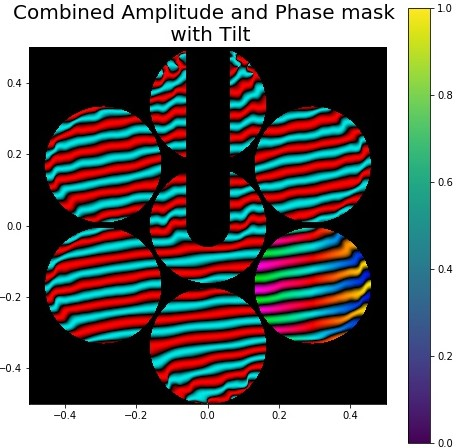
\includegraphics[width=6.5cm]{Figures/tilt_comb.jpg}
  \caption{Pupil image with induced tilt aberration}
  \label{fig:tilt_pupil}
\end{subfigure}%
\begin{subfigure}{.5\textwidth}
  \centering
  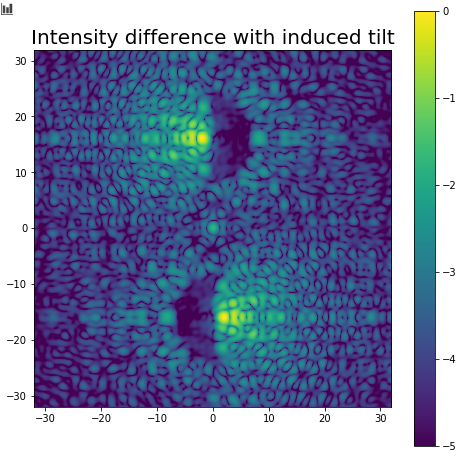
\includegraphics[width=6.5cm]{Figures/PSF_tilt.png}
  \caption{Log scale of focal plane with tilt aberration.}
  \label{fig:tilt_focal}
\end{subfigure}
\caption{Pupil and Focal plane of tilt applied to segment 4.}
\label{fig:abb_images}
\end{figure}

Last step is to find the response in the focal plane for this aberration.  This is simply done by repeating this
process but instead changing Equation \ref{eq:OPD} to have a negative OPD applied to it.  So the equation now
becomes $\phi = -2 \pi / \lambda$.  After repeating the process, we get a new focal plane image.  Now the response
for a tilt on segment 4 can be calculated by taking $I_{pos} - I_{neg}$ (Figure \ref{fig:I_diff}).  This image is
stored as a 1-D vector and all 21 combinations of P/T/T for each of the seven segments are stored in a matrix.  This
is our Response Matrix.  Now that there is a RM, we want to create the inverse of this matrix so that an inputted
aberration can output an amplitude of each mode in our modal basis set (P/T/T).  For a full array of response matrix images please refer to Appendix \ref{AppendixA}.


\begin{figure}[H]
    \centering
    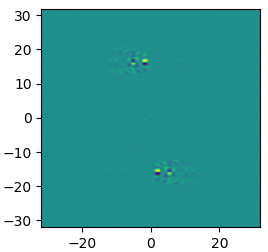
\includegraphics[width = 6cm]{Figures/I_diff.png}
    \caption{Focal plane response for tilt on segment 4.}
    \label{fig:I_diff}
\end{figure}



\section{Control Matrix}

Construction of the control matrix involves taking a pseudo-inverse of the RM.  This is done using singular value
decomposition of the RM.  Singular value decomposition (SVD) in linear algebra, is a way of decomposing a real or
complex square matrix into the pseudoinverse of a matrix \cite{Hestenes1958InversionResults}.  First we decompose
our response matrix $M$ into $M = U \Sigma V^{\ast}$ and the pseudoinverse is:

\begin{equation}
    M^{\dagger} = V \Sigma^{\dagger} U^{\ast}
    \label{eq:SVD}
\end{equation}

\begin{figure}[H]
    \centering
    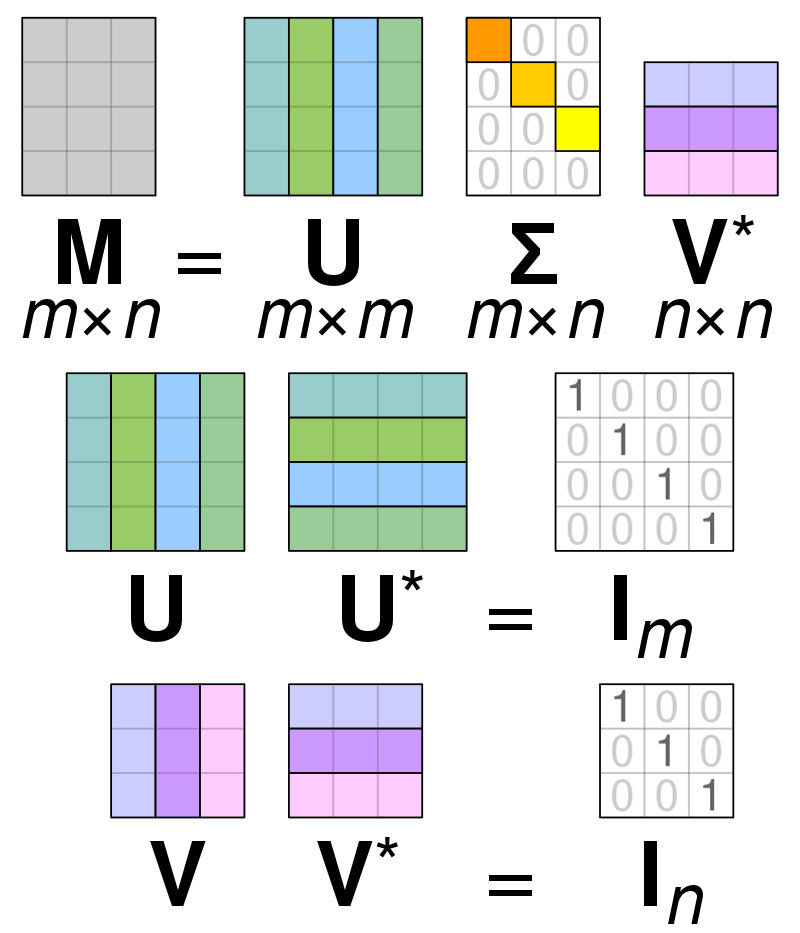
\includegraphics[width = 6cm]{Figures/Singular_value_decomposition_visualisation.jpg}
    \caption{A visual of Singular Value Decomposition}
    \label{fig:SVD}
\end{figure}

Where $\Sigma^{\dagger}$ is the pseudoinverse of $\Sigma$.  This is formed by replacing every non-zero diagonal entry by
its reciprocal and transposing the resulting matrix \cite{Hestenes1958InversionResults}.  A visual example of this
process can be seen in Figure \ref{fig:SVD}. Luckily all this complicated matrix inversion is simply done in HCIpy using
the function $inverse\_tikhonov$ \cite{por2018hcipy}.  However, to test the inversion of the matrix, I plotted the
singular values $\Sigma$ and compared them to previous values calculated (Figure \ref{fig:SV}).




\begin{figure}[H]
    \centering
    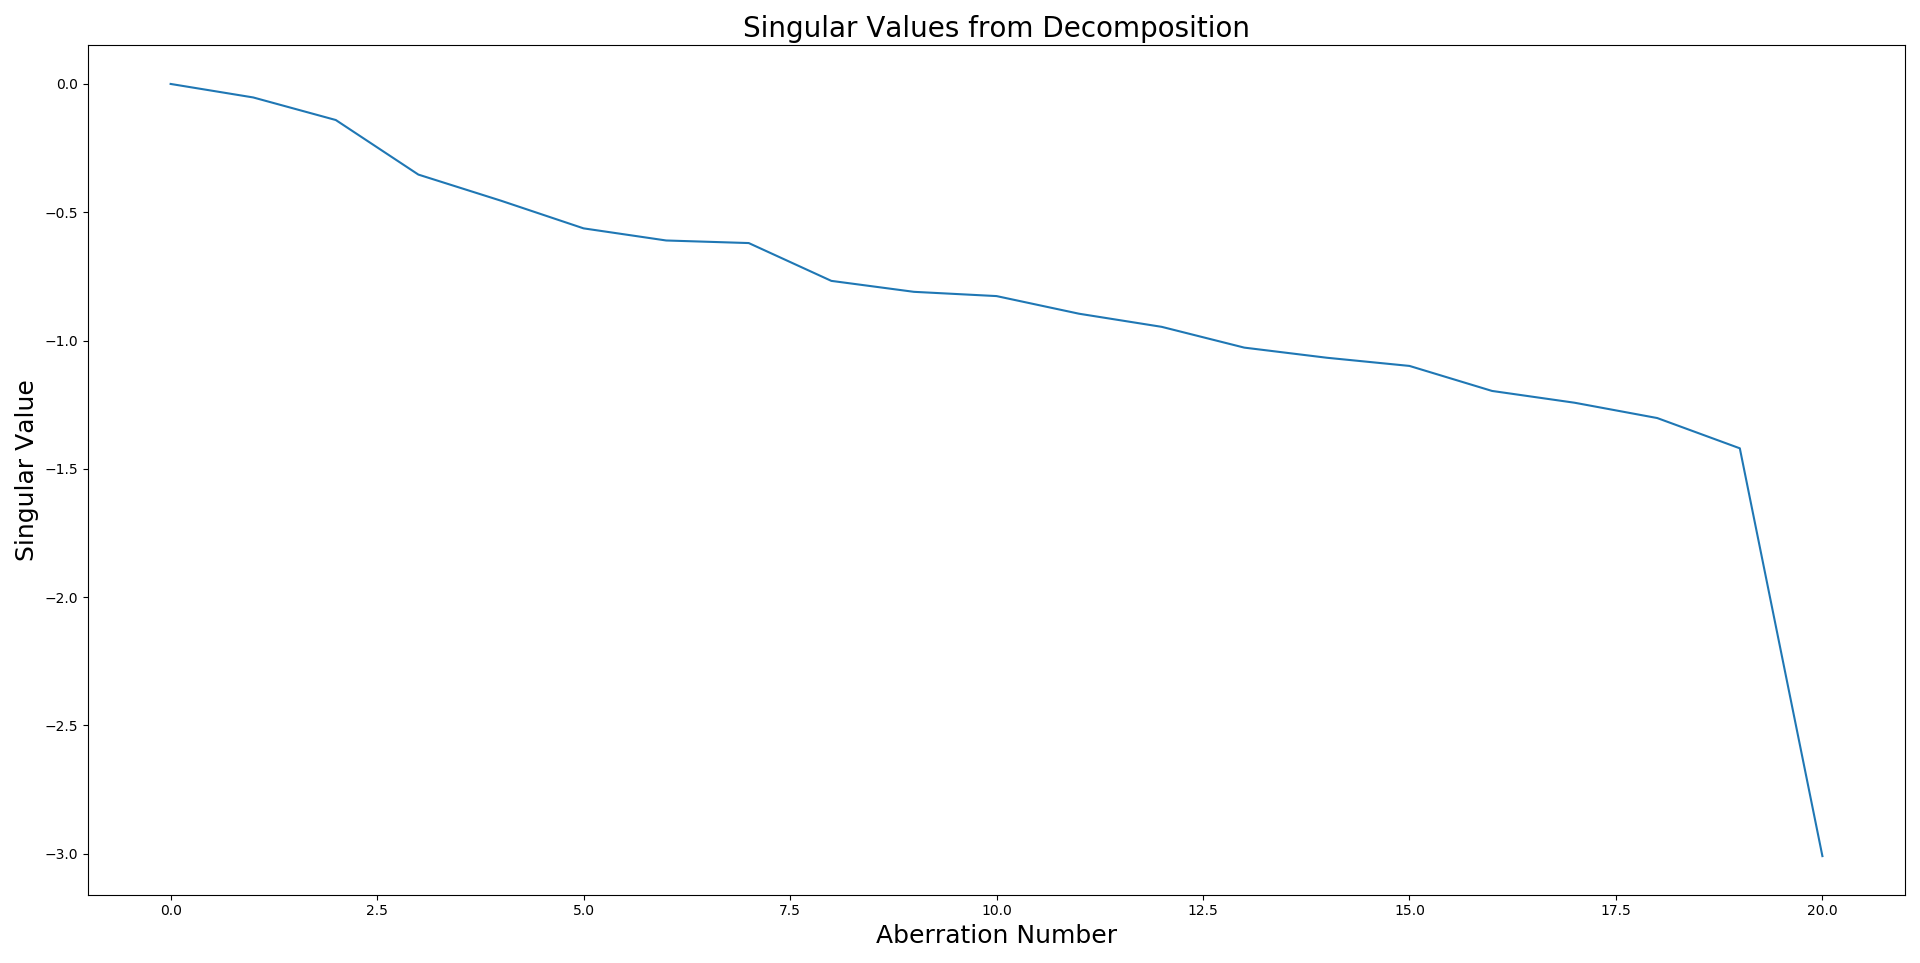
\includegraphics[width = 14cm]{Figures/singular_values.png}
    \caption{Singular Values of the Control Matrix}
    \label{fig:SV}
\end{figure}


The singular values were confirmed to match previous versions of other response matrices made for the GMT.  Therefore, we could move on to testing the wavefront sensing ability of our system.  To test this, we first take a reference image of an unaberrated focal plane and subtract that from an aberrated image.  The left over image is a residual intensity between the two images.  With that image, we can take the dot product of the control matrix and the residual image to get the amplitudes of all the modal basis set.  The results of this will be discussed in Chapter \ref{Chapter4}.  Now that we have shown that we can do focal plane wavefront sensing with a vAPP, we can go on to physically demonstrating it.
